\chapter{Related Works}
\label{Related Works}

\section{Standard Lane Following Algorithm}
As autonomous cars evolve into reality, there is a need for algorithms
to assist them in navigating and staying inside the lines. These
algorithms detect lines on the pavement, and
instructing the car to stay in the center. This is similar to
a two line crosswalk, the goal is to keep the user between the two
lines. However, with a crosswalk, the goal is to keep them inside the crosswalk, not necessarily centered.
One algorithm for lane following is as follows:
\begin{enumerate}
  \item Convert the image to grayscale
  \item Crop to the center portion of the image
  \item Identify the edges using an edge detection algorithm, and then draw the
  edges onto a new image
  \item Apply Hough line detection to find shapes in the edges \cite{HoughTransform}
  \item Delete extraneous lines that were detected
  \item Apply and draw the discovered lines on the main image
\end{enumerate}
By following these steps, the image is processed and the lanes are returned,
which can then be used to direct the car to remain inside the lane \cite{SingleLane1}.


%https://www.researchgate.net/publication/4207389_Bipolarity_and_Projective_Invariant-Based_Zebra-Crossing_Detection_for_the_Visually_Impaired

\section{Crosswalk Detection Approach Using Pixel Bipolarity}

Kyoto Institute of Technology's Uddin and Shioyama created a method of detecting zebra crosswalks using their geometric properties and the bipolarity of the images \cite{relatedworkbipolarity}. Their paper focuses on grouping large areas together that have high values of dark and/or light inside of them. Also, they use the projective invariant aka cross product to determine if the areas of light and dark in their image fit the pattern of a crosswalk. They then use the Fischer criterion to extract feature points in the image where the change from white to black (and vice versa) occur.

The steps are as follows:
\begin{enumerate}
   \item Convert to grayscale and split the image into 16x16 pixel groups.
   \item Find regions that are strongly bipolar by merging pixel groups that have a distance ratio within a threshold. The distance ratio is a measure of how similar the regions intensities are to each other in regards to bipolarity. A merged image is shown in figure \ref{fig:BipolarCrosswalk} section  (b).
   \item Once grouped, discard regions that don't exhibit enough bipolarity.
   \item Refine the segmentation by allowing larger groups to absorb smaller groups inside of them.
   \item Check where the region is in the image. If it is far to the left or right, classify it as such. If the bottom of the region is too high up in the image, discard it.
   \item Use a Fourier transform to check if the crosswalk angle is too extreme. If it is, throw it out. 
   \item Use Fischer criteria to find the feature points where the intensity changes drastically, determine that there are at least seven (which means there are four or more crosswalk stripes in the image), and then check the projective invariant criteria to see if it passes or is thrown out\cite{relatedworkbipolarity}. 
   \item Repeat for each region until a match is found or all regions are exhausted.
\end{enumerate}
This method had decent results, with a high true positive rate (74 / 79), and zero false positives out of 34 other images. One downside of their method is that the image is required to have a minimum of four crosswalk stripes in the image to detect it, which means the majority of the crosswalk must be in the frame. Theoretically this method will work with a moderate amount of the crosswalk covered up (by other pedestrians or cars) as long as there are enough feature points in a vertical line in at least one area to detect the crosswalk. 

\begin{figure}[t]
\begin{center}
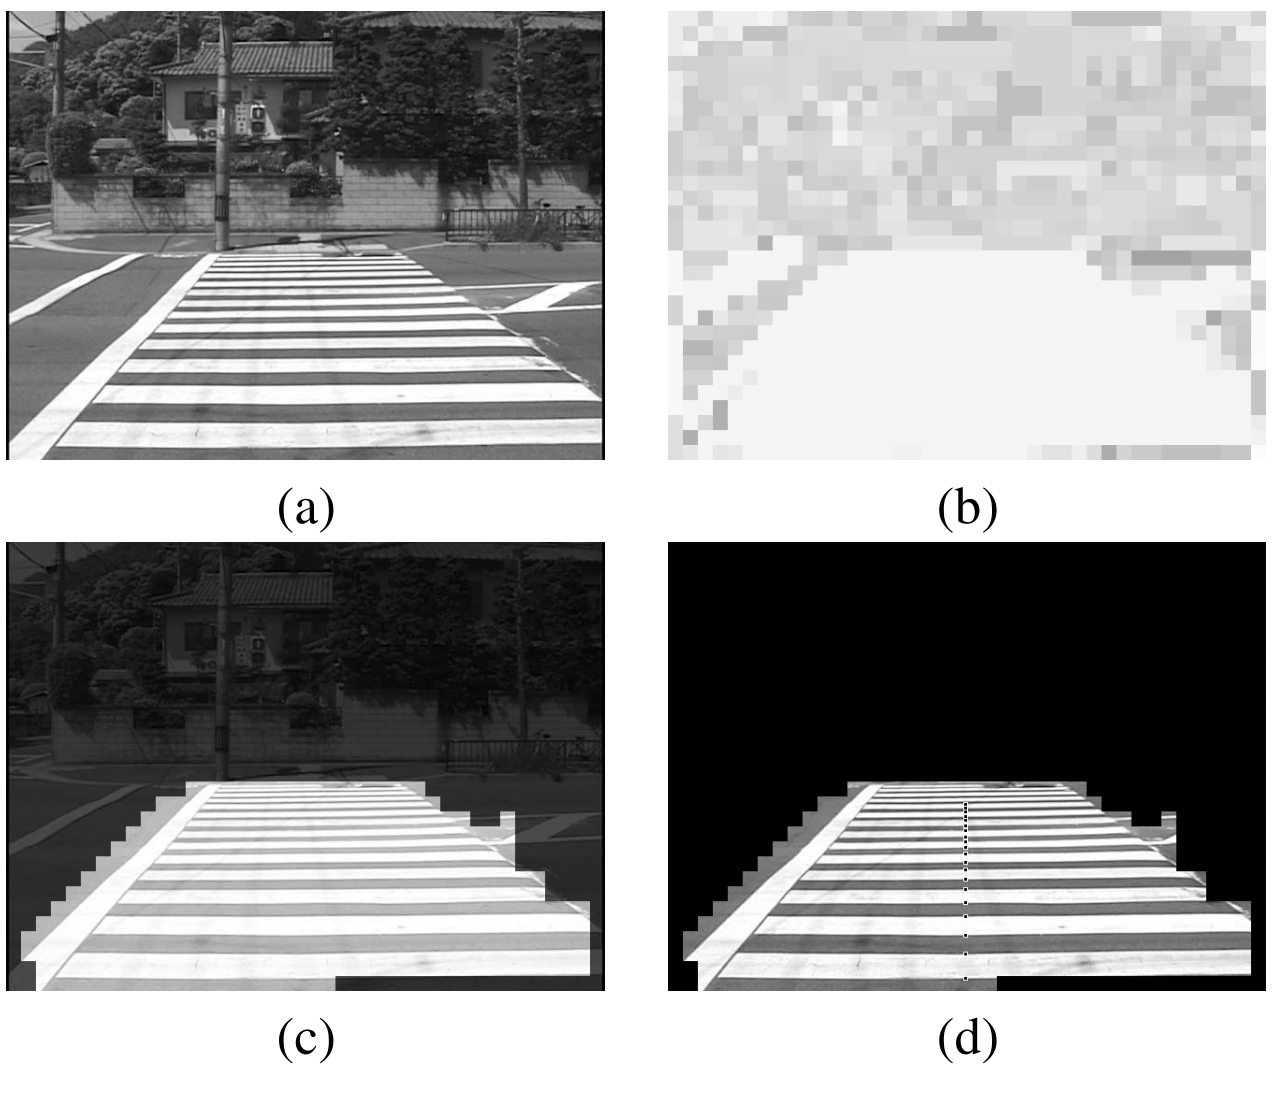
\includegraphics[width=10cm]{figures/BipolarCrosswalk.png}
\captionfonts
\caption{Steps of detecting a zebra crosswalk using Bipolarity and Projective Invariant: (a) gray scale image, (b) bipolarity of each segmented region, (c) original image highlighting the largest detected region, (d) extracted feature points shown on region}
\label{fig:BipolarCrosswalk}
\end{center}
\end{figure}
